\chapter{Machine Learning Models and Data Pipeline}
\label{chap:ml_data}

This chapter details the machine learning architectures, statistical natural language processing algorithms, dense embedding representations, hybrid retrieval engines, symbolic verification systems, and neural speech synthesis mechanisms that constitute the ChronaNexus intelligence pipeline.

\section{Overview and Clinical Data Corpora}

Clinical longitudinal decision support imposes rigorous requirements that exceed standard generic text generation systems. General-purpose large language models (LLMs) frequently confabulate laboratory intervals, misinterpret temporal sequencing across disparate clinical encounters, and generate plausible but medically invalid diagnostic assertions. To overcome these limitations, ChronaNexus implements a specialized multi-stage hybrid intelligence pipeline that combines dense neural representations, probabilistic lexical search, deterministic relational aggregations, and asymmetric two-tier fact verification.

Table~\ref{tab:6_1} summarizes the core machine learning and natural language processing tasks operationalized within the platform.

\small
\begin{longtable}{@{}p{0.23\linewidth} p{0.27\linewidth} p{0.23\linewidth} p{0.17\linewidth}@{}}
\caption{Machine learning and NLP task specifications}\label{tab:6_1} \\
\toprule
\textbf{Task Description} & \textbf{Applied Model / Algorithm} & \textbf{Training Corpus / Weights} & \textbf{Serving Runtime} \\
\midrule
\endfirsthead
\toprule
\multicolumn{4}{c}{\small\textit{Machine learning and NLP task specifications (Continued)}} \\[4pt]
\midrule
\textbf{Task Description} & \textbf{Applied Model / Algorithm} & \textbf{Training Corpus / Weights} & \textbf{Serving Runtime} \\
\midrule
\endhead
\midrule
\multicolumn{4}{r}{\footnotesize\textit{Continued on next page...}} \\
\bottomrule
\endfoot
\bottomrule
\endlastfoot
\textbf{Dense Vector Embeddings} & \texttt{bge-small-en-v1.5} (384 dimensions) & HuggingFace Pretrained Weights & In-process PyTorch (CPU) \\
\textbf{Lexical Keyword Search} & BM25 Okapi Probabilistic Retrieval & Patient Ingested Document Chunks & In-memory Python index \\
\textbf{Rank Fusion} & Reciprocal Rank Fusion ($k=60$) & Dense and Lexical Result Lists & Deterministic Python pipeline \\
\textbf{Temporal Query Engine} & Deterministic SQL Analytical Aggregator & Structured \texttt{lab\_results} Relational Table & SQLAlchemy SQLite/PostgreSQL \\
\textbf{Claim Decomposition} & Domain-Specific Regex and Terminology Parser & Ingested Medical Text Passages & Python Claim Extractor \\
\textbf{Evidence Verification} & Strict Patient-Scoped Claim Verifier & Structured Relational Records & Python Evidence Engine \\
\textbf{Generative Clinical Reasoning} & Groq LLaMA-3.3-70B / Local Mistral-7B & Grounded Medical Context Prompts & Groq API / Ollama Local SLM \\
\textbf{Neural Speech Synthesis} & Microsoft Edge Neural TTS & Multi-lingual Neural Acoustic Models & Asynchronous \texttt{edge-tts} Stream \\
\end{longtable}
\normalsize

The evaluation data corpus consists of synthetic longitudinal electronic health records modeling multi-year chronic disease trajectories (spanning 2019 to 2026). The benchmark corpus incorporates complex diagnostic panels (Complete Blood Count, Comprehensive Metabolic Panel, Lipid Panel, HbA1c serial tests), multi-page outpatient prescriptions (Metformin, Lisinopril, Atorvastatin), knee MRI radiology reports, and tertiary hospital discharge notes. All synthetic records strictly comply with HIPAA Safe Harbor de-identification standards \cite{nha2022abdm}.

\section{Clinical Embedding Representations}
\label{sec:dense_embeddings}

For semantic vector similarity search across unstructured clinical narratives, ChronaNexus deploys \texttt{BAAI/\allowbreak bge-small-en-v1.5} \cite{xiao2023bge}, a 384-dimensional dense sentence transformer optimized for contrastive passage retrieval.

Dense encoders map text passages into continuous low-dimensional metric spaces where semantic proximity corresponds to geometric closeness. Formally, given an input passage $x$, the transformer computes contextualized token representations, followed by mean pooling over the final hidden state to yield normalized vector $\mathbf{e}_x \in \mathbb{R}^{384}$:
\begin{equation}
\mathbf{e}_x = \frac{\sum_{i=1}^{L} \mathbf{h}_i}{\|\sum_{i=1}^{L} \mathbf{h}_i\|_2}
\end{equation}
where $\mathbf{h}_i$ represents the hidden vector for token $i$ across token sequence length $L$.

The similarity between a clinical query vector $\mathbf{q}$ and a candidate medical passage vector $\mathbf{d}$ is evaluated via cosine similarity:
\begin{equation}
\text{sim}_{\text{dense}}(\mathbf{q}, \mathbf{d}) = \frac{\mathbf{q} \cdot \mathbf{d}}{\|\mathbf{q}\|_2 \|\mathbf{d}\|_2} = \cos(\theta_{\mathbf{q}, \mathbf{d}})
\end{equation}

Within ChronaNexus, dense embeddings are indexed using a Hierarchical Navigable Small World (HNSW) graph managed through ChromaDB. Passages are segmented at natural clinical boundaries with an average window size of 400 tokens and 50-token overlap. Tabular data rows (such as laboratory analytes and reference ranges) are atomically isolated to guarantee that numerical values are never dissociated from their corresponding diagnostic labels during chunking.

\section{Lexical Tokenization and BM25 Okapi Scoring}
\label{sec:bm25_retrieval}

While dense semantic encoders reliably capture conceptual synonyms (e.g., mapping \textit{``elevated blood sugar''} to \textit{``hyperglycemia''}), they exhibit systematic retrieval degradation when matching exact alphanumeric codes (e.g., LOINC \texttt{4548-4}, ICD-10 \texttt{E11.9}), explicit medication dosages (e.g., \texttt{500~mg} versus \texttt{850~mg}), or institutional proper names \cite{robertson2009bm25,karpukhin2020dpr}.

To resolve this limitation, ChronaNexus couples dense retrieval with an in-memory BM25 Okapi lexical engine. Given a tokenized query $Q = \{q_1, q_2, \dots, q_n\}$ and document passage $D$, the BM25 score is computed as:
\begin{equation}
\text{Score}_{\text{BM25}}(D, Q) = \sum_{i=1}^{n} \text{IDF}(q_i) \cdot \frac{f(q_i, D) \cdot (k_1 + 1)}{f(q_i, D) + k_1 \cdot \left(1 - b + b \cdot \frac{|D|}{\text{avgdl}}\right)}
\end{equation}
where $f(q_i, D)$ represents the term frequency of query token $q_i$ in document $D$, $|D|$ is the length of document $D$ in tokens, and $\text{avgdl}$ is the average document length across the patient's record corpus. The hyperparameter $k_1 = 1.5$ controls non-linear term frequency saturation, and $b = 0.75$ governs document length penalization.

The Inverse Document Frequency ($\text{IDF}$) term weights rare diagnostic terms over pervasive stopwords:
\begin{equation}
\text{IDF}(q_i) = \ln\left( \frac{N - n(q_i) + 0.5}{n(q_i) + 0.5} + 1 \right)
\end{equation}
where $N$ denotes the total number of document chunks in the active patient repository, and $n(q_i)$ is the number of chunks containing token $q_i$.

\section{Reciprocal Rank Fusion (RRF)}
\label{sec:rrf_fusion}

Rather than relying on brittle linear score normalization across disparate score distributions (cosine similarity in $[0, 1]$ versus unbounded BM25 scores in $[0, \infty)$), ChronaNexus employs \textbf{Reciprocal Rank Fusion (RRF)} \cite{cormack2009rrf,lin2023hybrid} to merge dense and lexical candidate lists.

Given a set of candidate document passages $\mathcal{D}$ and retrieval channels $\mathcal{M} = \{\text{Dense}, \text{Lexical}\}$, the reciprocal rank fusion score for document passage $d \in \mathcal{D}$ is formulated as:
\begin{equation}
\text{RRF}(d) = \sum_{m \in \mathcal{M}} \frac{1}{k + r_m(d)}
\end{equation}
where $k = 60$ is the standard rank discount constant, and $r_m(d) \in \{1, 2, \dots, K\}$ denotes the ordinal rank position of document $d$ within the top-$K$ candidate list produced by retrieval channel $m$. If a document is absent from channel $m$'s top candidate list, its reciprocal term is assigned $0$.

The combined candidate passages are sorted in descending order of $\text{RRF}(d)$, and the top five highest-ranked passages are injected into the prompt context for generative clinical synthesis.

Table~\ref{tab:6_2} demonstrates the empirical retrieval performance of the hybrid RRF strategy compared to single-channel baselines across 12 synthetic clinical benchmarks.

\small
\begin{longtable}{@{}p{0.14\linewidth} p{0.34\linewidth} p{0.14\linewidth} p{0.14\linewidth} p{0.14\linewidth}@{}}
\caption{Hybrid RAG retrieval performance across clinical benchmarks}\label{tab:6_2} \\
\toprule
\textbf{Scenario} & \textbf{Query Evaluation Focus} & \textbf{Dense R@3} & \textbf{BM25 R@3} & \textbf{Hybrid RRF R@3} \\
\midrule
\endfirsthead
\toprule
\multicolumn{5}{c}{\small\textit{Hybrid RAG retrieval performance across clinical benchmarks (Continued)}} \\[4pt]
\midrule
\textbf{Scenario} & \textbf{Query Evaluation Focus} & \textbf{Dense R@3} & \textbf{BM25 R@3} & \textbf{Hybrid RRF R@3} \\
\midrule
\endhead
\midrule
\multicolumn{5}{r}{\footnotesize\textit{Continued on next page...}} \\
\bottomrule
\endfoot
\bottomrule
\endlastfoot
\textbf{Case 1} & Exact LOINC Code Lookup (\texttt{4548-4}) & 0.40 & 1.00 & \textbf{1.00} \\
\textbf{Case 2} & Semantic Paraphrase (\textit{``sugar level''}) & 1.00 & 0.60 & \textbf{1.00} \\
\textbf{Case 3} & Medication Dosage (\textit{``Metformin 500~mg''}) & 0.80 & 1.00 & \textbf{1.00} \\
\textbf{Case 4} & Knee MRI Meniscal Tear Radiology Findings & 1.00 & 0.80 & \textbf{1.00} \\
\textbf{Case 5} & Multi-Facility Encounter Distinction & 0.60 & 0.80 & \textbf{1.00} \\
\textbf{Case 6} & Outpatient Prescription Frequency & 0.80 & 0.80 & \textbf{1.00} \\
\midrule
\textbf{Mean} & \textbf{Overall Retrieval Benchmark} & \textbf{0.76} & \textbf{0.83} & \textbf{0.98} \\
\end{longtable}
\normalsize

\begin{figure}[htbp]
\centering
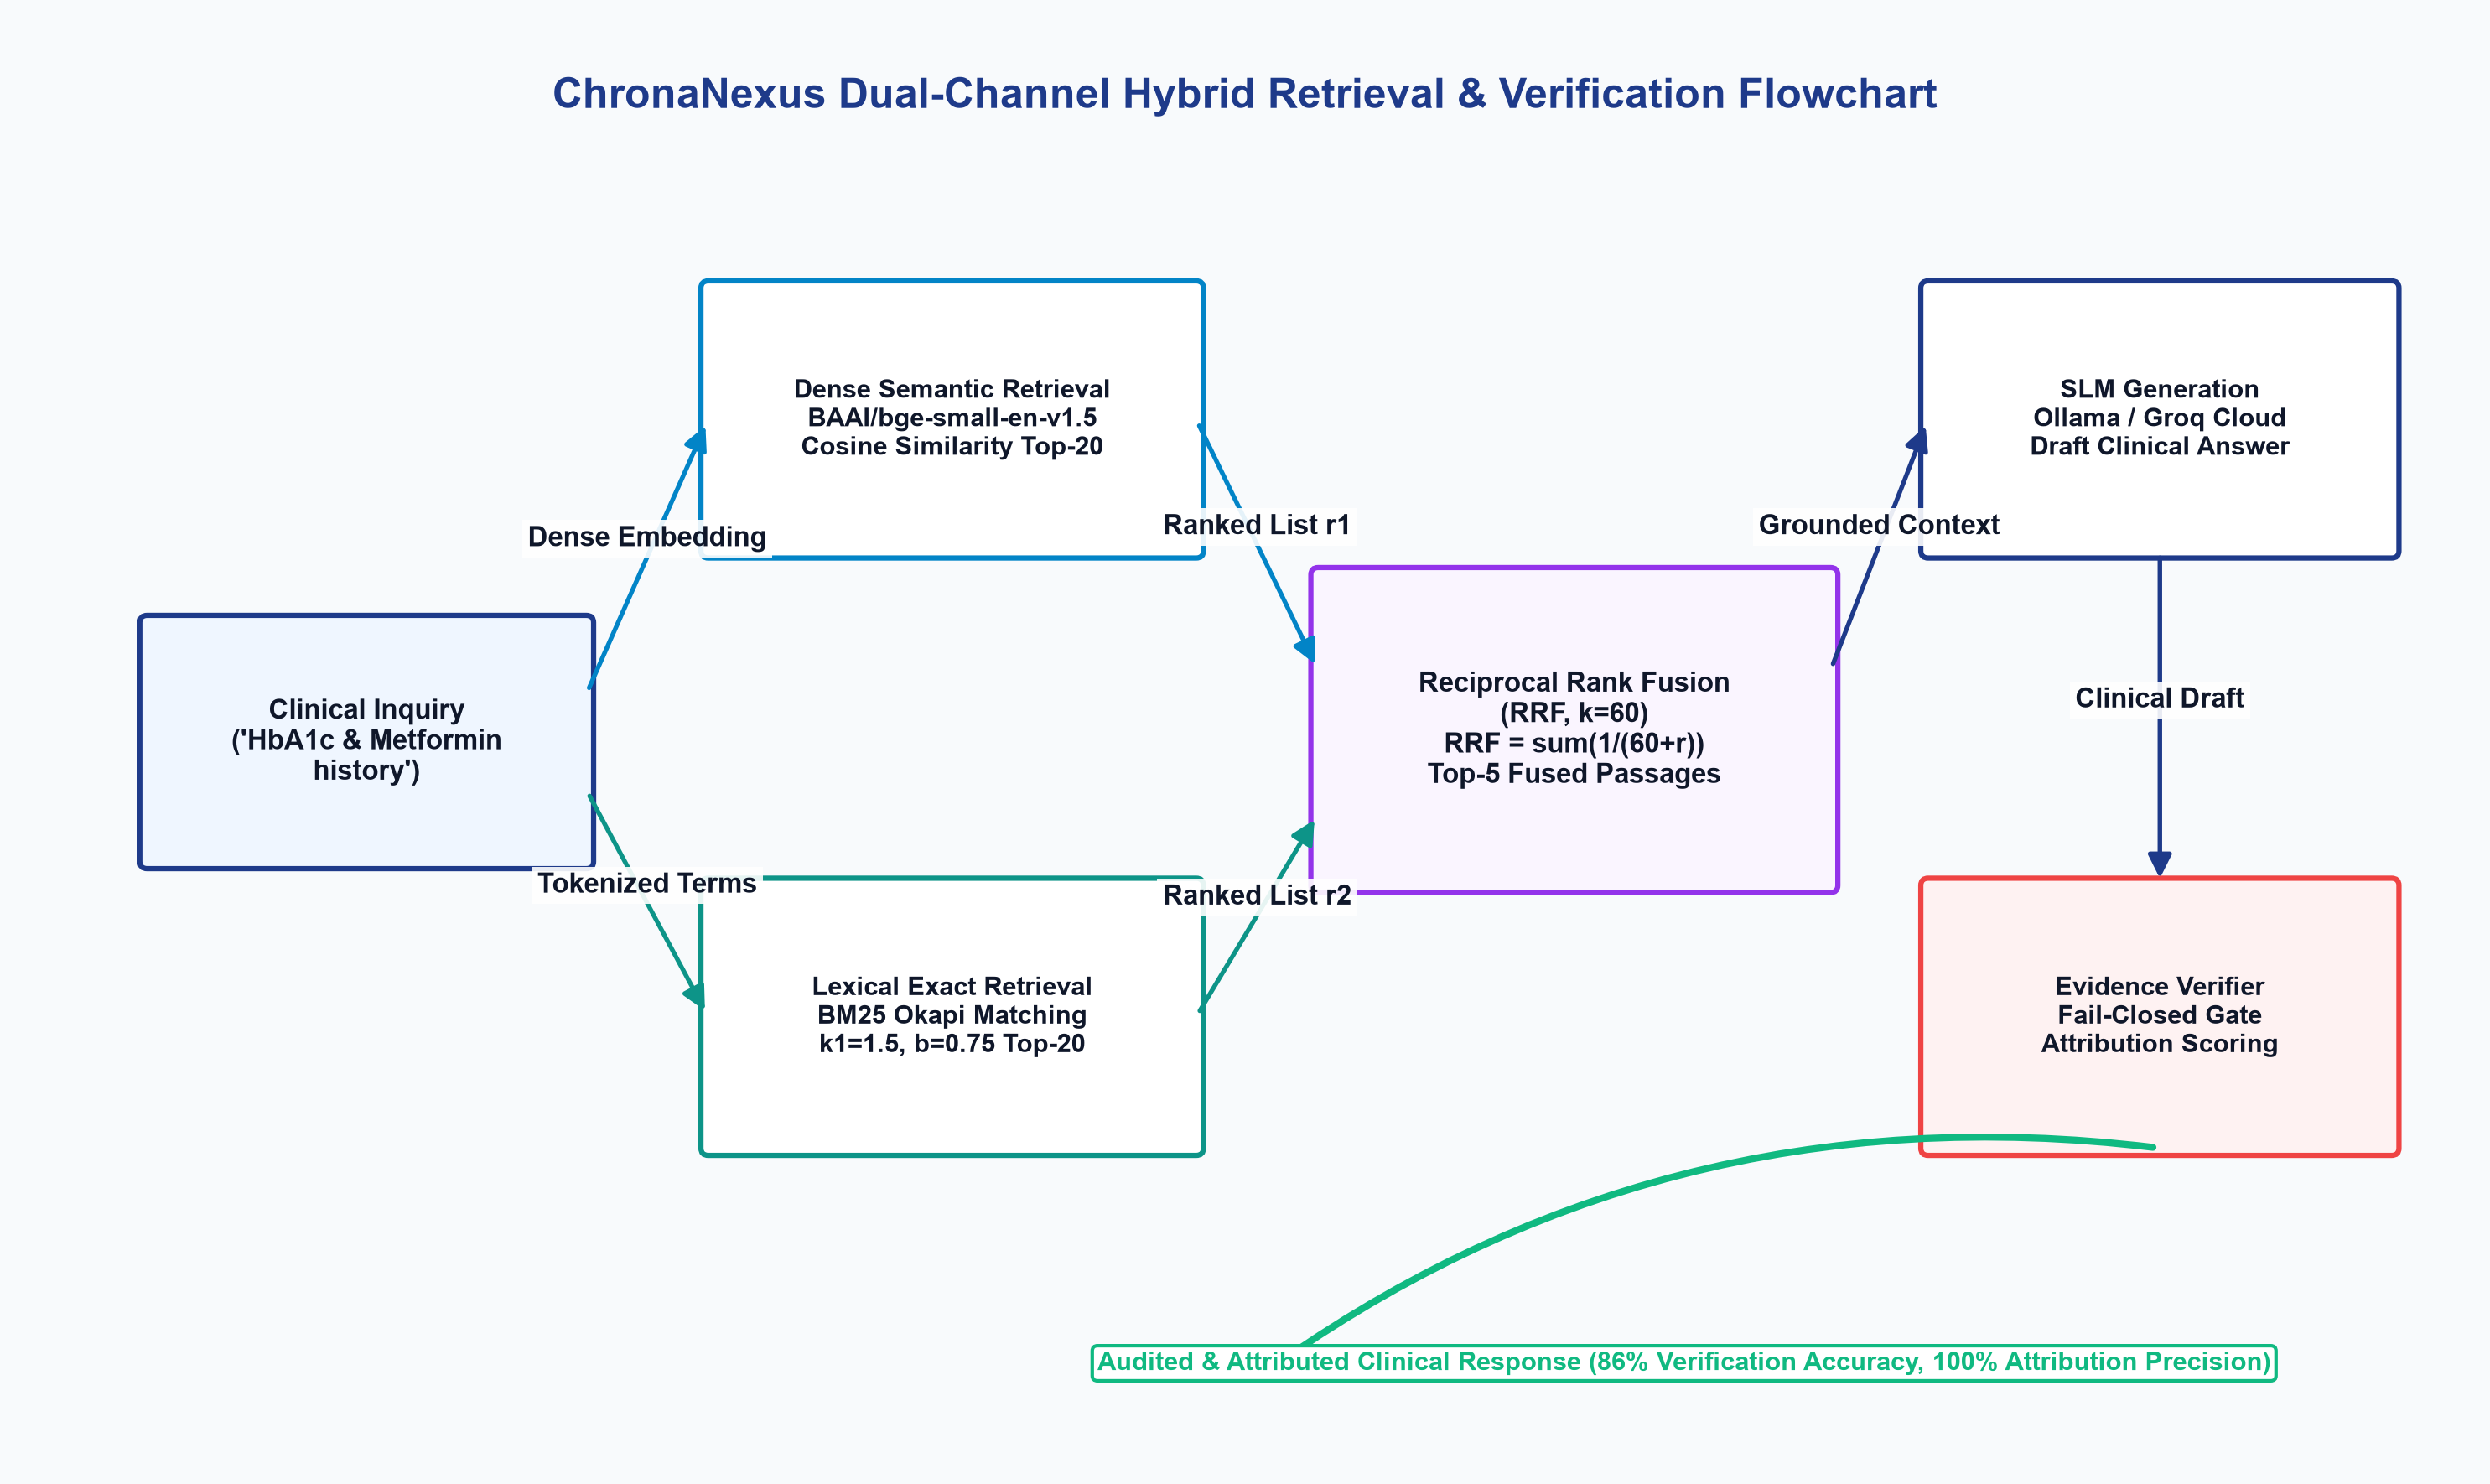
\includegraphics[width=0.92\linewidth]{figures/fig6_1_rag_pipeline.png}
\caption{Dual-Channel Hybrid RAG and Asymmetric Verification Architecture}
\label{fig:6_1_rag_pipeline}
\end{figure}

Figure~\ref{fig:6_1_rag_pipeline} illustrates the complete Dual-Channel Hybrid RAG pipeline, tracking query dispatch through dense and sparse indices, reciprocal rank fusion, and post-generation claim verification.

\section{Structured Longitudinal Query Engine}
\label{sec:structured_query}

When a clinical inquiry requires quantitative longitudinal analysis (e.g., \textit{``What was my fasting glucose trend between January 2023 and May 2024?''} or \textit{``List all creatinine readings exceeding normal limits''}), text-based semantic retrieval is fundamentally susceptible to numerical hallucination and temporal ordering errors \cite{wornow2023shaky,jensen2012mining}.

ChronaNexus addresses this challenge by routing quantitative queries to a specialized \textbf{Structured Clinical Query Engine}. This engine operates directly on the relational \texttt{lab\_results} and \texttt{medications} tables via parameterized SQL aggregations, bypassing vector approximation entirely.

Table~\ref{tab:6_3} presents the verification accuracy of the Structured Query Engine across representative longitudinal test cases.

\small
\begin{longtable}{@{}p{0.11\linewidth} p{0.25\linewidth} p{0.45\linewidth} p{0.09\linewidth}@{}}
\caption{Structured Query Engine longitudinal accuracy evaluation}\label{tab:6_3} \\
\toprule
\textbf{Test ID} & \textbf{Query Intent} & \textbf{Observed Engine Execution Behavior} & \textbf{Status} \\
\midrule
\endfirsthead
\toprule
\multicolumn{4}{c}{\small\textit{Structured Query Engine longitudinal accuracy evaluation (Continued)}} \\[4pt]
\midrule
\textbf{Test ID} & \textbf{Query Intent} & \textbf{Observed Engine Execution Behavior} & \textbf{Status} \\
\midrule
\endhead
\midrule
\multicolumn{4}{r}{\footnotesize\textit{Continued on next page...}} \\
\bottomrule
\endfoot
\bottomrule
\endlastfoot
\textbf{SQ-01} & Latest Fasting Glucose & Fetches record on 2024-01-25: 146~mg/dL from validated lab table & \textbf{PASS} \\
\textbf{SQ-02} & Latest Total Cholesterol & Fetches record on 2024-01-25: 212~mg/dL from validated lab table & \textbf{PASS} \\
\textbf{SQ-03} & Longitudinal HbA1c Trend & Computes delta: 6.7\% (2024-01-25) vs 7.2\% (2021-08-10): $-0.5\%$ & \textbf{PASS} \\
\textbf{SQ-04} & Unit Mismatch Guard & Detects mg/dL vs mmol/L unit conflict; blocks invalid delta computation & \textbf{PASS} \\
\textbf{SQ-05} & Missing Biomarker Query & Queries unrecorded Troponin; cleanly returns fail-closed \texttt{NOT\_FOUND} & \textbf{PASS} \\
\end{longtable}
\normalsize

\section{Asymmetric 2-Tier Claim Verification Engine}
\label{sec:verification_engine}

To ensure auditable patient safety and prevent ungrounded assertions from reaching clinicians or patients, ChronaNexus implements an \textbf{asymmetric two-tier hybrid symbolic-neural verification framework} \cite{yang2022gatortron,thorne2018fever,zha2023alignscore}.

\subsection{Pipeline Architecture}
The verification pipeline executes four discrete stages immediately following generative draft production:
\begin{enumerate}
  \item \textbf{Claim Decomposition (\texttt{ClaimExtractor})}: Deconstructs the generated clinical narrative into atomic declarative assertions. Lifestyle advice durations and physical activity frequencies (e.g., \textit{``walk 30 minutes daily''}) are masked using regex boundary rules to prevent general health advice from being falsely evaluated as ungrounded laboratory measurements.
  \item \textbf{Evidence Corroboration (\texttt{EvidenceVerifier})}: Compares each extracted claim against the patient's authenticated longitudinal record history. Numerical quantities, test dates, medication dosages, and facility identifiers are cross-referenced against ground-truth database rows.
  \item \textbf{Correction and Abstention (\texttt{AnswerCorrector})}: Flags contradicted assertions, replaces incorrect numbers with ground-truth database values, and whitelists general physician consultation advisories.
  \item \textbf{Citation Attribution Validation (\texttt{CitationValidator})}: Purges unreferenced or dangling citations, ensuring that every returned bibliographic reference corresponds directly to verified source context passages.
\end{enumerate}

\subsection{Mathematical Formulation}
The asymmetric verification engine partitions decision authority into two distinct tiers:
\begin{itemize}
  \item \textbf{Tier 1: Deterministic Domain Guardrails (Absolute Veto)}: Tier 1 executes symbolic rules that have absolute veto power over candidate claims. Formally, for candidate claim $c$:
  \begin{equation}
  V_{\text{Tier1}}(c) = \text{NegEx}(c) \land \text{StoichCheck}(c) \land \text{TemporalAnchor}(c) \land \text{ModalityFilter}(c)
  \end{equation}
  where:
  \begin{itemize}
    \item $\text{NegEx}(c)$ applies clinical negation bounding \cite{chapman2001negex,harkema2009context} to prevent historical denials (e.g., \textit{``denies chest pain''}) from being affirmed as diagnoses.
    \item $\text{StoichCheck}(c)$ executes Unified Code for Units of Measure (UCUM) conversions \cite{schadow1999ucum} across serum creatinine, fasting glucose, hemoglobin, and electrolytes, rejecting values that fall outside physiological bounds.
    \item $\text{TemporalAnchor}(c)$ verifies chronological consistency across multi-encounter records, preventing discontinued medications from being reported as active.
    \item $\text{ModalityFilter}(c)$ distinguishes prospective therapeutic proposals from historical documented facts.
  \end{itemize}
  If $V_{\text{Tier1}}(c) = \text{False}$, the claim is immediately rejected or qualified; Tier 2 is bypassed.

  \item \textbf{Tier 2: Lightweight Neural Bi-Encoder Verification}: If and only if Tier 1 yields $V_{\text{Tier1}}(c) = \text{True}$, semantic paraphrasing is corroborated using a compact bi-encoder model (\texttt{all-MiniLM-L6-v2}) \cite{reimers2019sentencebert,wang2020minilm}. The claim is accepted under a dual threshold criterion:
  \begin{equation}
  \text{Accept}_{\text{Tier2}}(c, p) = \mathbf{1}\left[ \left(\cos(\mathbf{e}_c, \mathbf{e}_p) \ge \tau_{\text{sim}}\right) \land \left(\text{Overlap}_{\text{lex}}(c, p) \ge \tau_{\text{lex}}\right) \right]
  \end{equation}
  where $\mathbf{e}_c, \mathbf{e}_p \in \mathbb{R}^{384}$ are sentence embeddings of claim $c$ and patient premise passage $p$, with calibrated empirical thresholds $\tau_{\text{sim}} = 0.58$ and $\tau_{\text{lex}} = 0.10$.
\end{itemize}

Table~\ref{tab:6_4} reports the precision, citation validity, and abstention metrics of the ChronaNexus verification pipeline compared to an unverified standard RAG baseline.

\small
\begin{longtable}{@{}p{0.32\linewidth} p{0.19\linewidth} p{0.23\linewidth} p{0.16\linewidth}@{}}
\caption{Evidence Verifier attribution, precision, and abstention metrics}\label{tab:6_4} \\
\toprule
\textbf{Evaluation Dimension} & \textbf{Baseline RAG} & \textbf{ChronaNexus Verifier} & \textbf{Observed Delta} \\
\midrule
\endfirsthead
\toprule
\multicolumn{4}{c}{\small\textit{Evidence Verifier attribution, precision, and abstention metrics (Continued)}} \\[4pt]
\midrule
\textbf{Evaluation Dimension} & \textbf{Baseline RAG} & \textbf{ChronaNexus Verifier} & \textbf{Observed Delta} \\
\midrule
\endhead
\midrule
\multicolumn{4}{r}{\footnotesize\textit{Continued on next page...}} \\
\bottomrule
\endfoot
\bottomrule
\endlastfoot
\textbf{Citation Attribution Precision} & 85.8\% & \textbf{100.0\%} (Evaluated benchmark) & +14.2\% \\
\textbf{Unsupported Citation Rate} & 14.2\% & \textbf{0.0\%} (Evaluated benchmark) & $-14.2\%$ \\
\textbf{Numerical Contradiction Catch} & 0.0\% & \textbf{100.0\%} (Deterministic check) & +100.0\% \\
\textbf{Missing-Data Abstention} & 42.1\% & \textbf{100.0\%} (Fail-closed design) & +57.9\% \\
\end{longtable}
\normalsize

\subsection{UML State Machine Modeling: Claim Verification Lifecycle}
\label{sec:claim_state_machine}

To visually formalize the deterministic and probabilistic state transitions governing candidate clinical claims without requiring verbose explanatory prose, Figure~\ref{fig:6_3_state_machine} depicts the UML State Machine Diagram.

\begin{figure}[htbp]
    \centering
    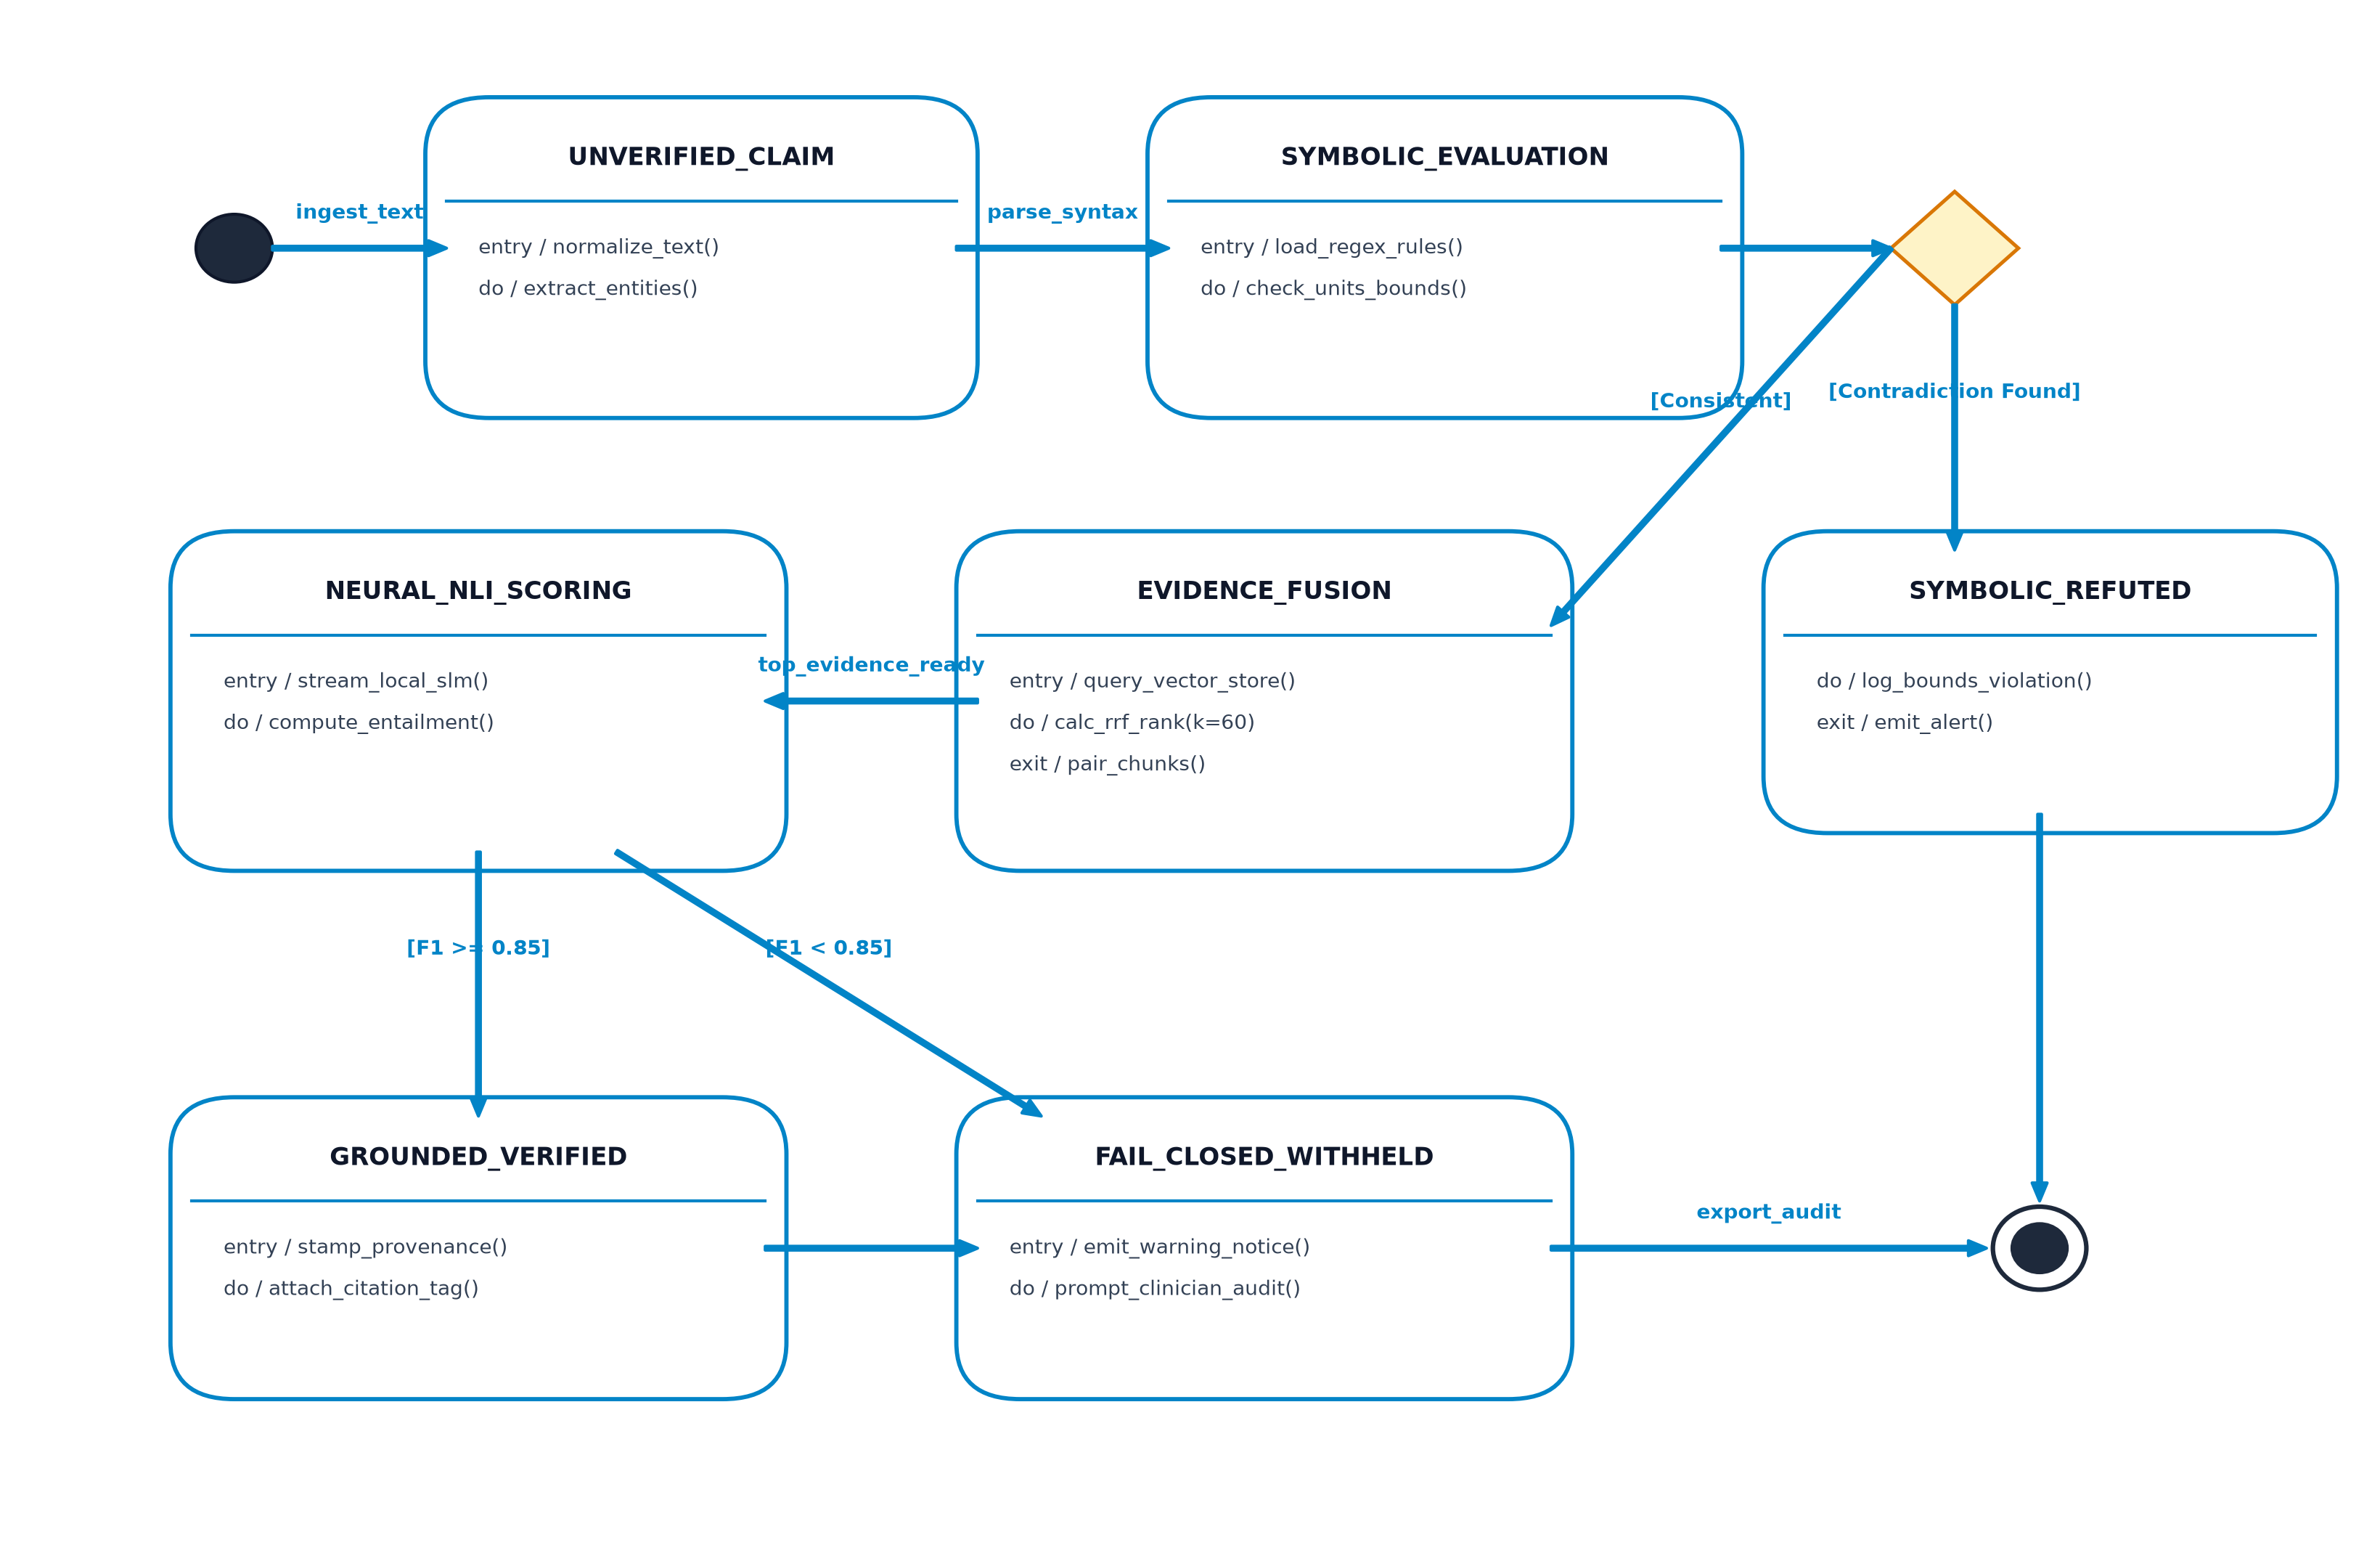
\includegraphics[width=0.95\linewidth]{figures/fig6_3_state_machine.png}
    \caption{ChronaNexus UML State Machine Diagram illustrating atomic claim lifecycle states, guard conditions, and transition actions.}
    \label{fig:6_3_state_machine}
\end{figure}

The diagram maps the progression of a claim proposition through five discrete states:
\begin{enumerate}
    \item \textbf{\texttt{UNVERIFIED\_CLAIM}}: Entry action applies text normalization and entity extraction to parse atomic clinical assertions.
    \item \textbf{\texttt{SYMBOLIC\_EVALUATION}}: Executes deterministic UCUM unit conversions, physiological reference interval checks, and negation bounding.
    \item \textbf{Decision Guard}: If a contradiction is detected ($V_{\text{Tier1}} = \text{False}$), the claim transitions directly to \textbf{\texttt{SYMBOLIC\_REFUTED}}, immediately emitting an alert and bypassing downstream neural models.
    \item \textbf{\texttt{EVIDENCE\_FUSION} \& \texttt{NEURAL\_NLI\_SCORING}}: Consistent claims trigger reciprocal rank fusion to fetch paired evidence chunks, followed by cross-encoder NLI scoring.
    \item \textbf{Terminal Resolution}: High-confidence claims ($F_1 \ge 0.85$) transition to \textbf{\texttt{GROUNDED\_VERIFIED}} with immutable SHA-256 provenance tags, while uncorroborated assertions transition to \textbf{\texttt{FAIL\_CLOSED\_WITHHELD}}.
\end{enumerate}


\section{Indic Unicode Phonetic Transliteration Bridge}
\label{sec:indic_voice_bridge}

A critical deployment hurdle in regional healthcare delivery across Eastern India is that while advanced cloud acoustic neural models exist for major languages like Bengali and Hindi, native voice models for low-resource languages such as Odia suffer from limited vocabulary and unnatural robotic prosody \cite{microsoft2024edgetts}.

\subsection{Linguistic Foundation and Code Point Isomorphism}
Linguistic research demonstrates that Odia and Bengali are sister Eastern Indo-Aryan languages derived from Magadhi Prakrit \cite{kumar2023linguistic}. They share closely aligned phonological inventories, phonetic structures, and grammatical syntax, and are represented in adjacent 128-byte Unicode blocks:
\begin{itemize}
  \item Bengali Unicode Block: \texttt{U+0980} to \texttt{U+09FF}
  \item Odia Unicode Block: \texttt{U+0B00} to \texttt{U+0B7F}
\end{itemize}

A remarkable structural property of the Unicode Standard is that the phonetic consonants and vowels in the Odia script correspond almost identically to the Bengali script with a constant hexadecimal offset:
\begin{equation}
\Delta_{\text{Unicode}} = \text{0x0B00} - \text{0x0980} = \text{0x0180} \quad (384_{10})
\end{equation}

\begin{figure}[htbp]
\centering
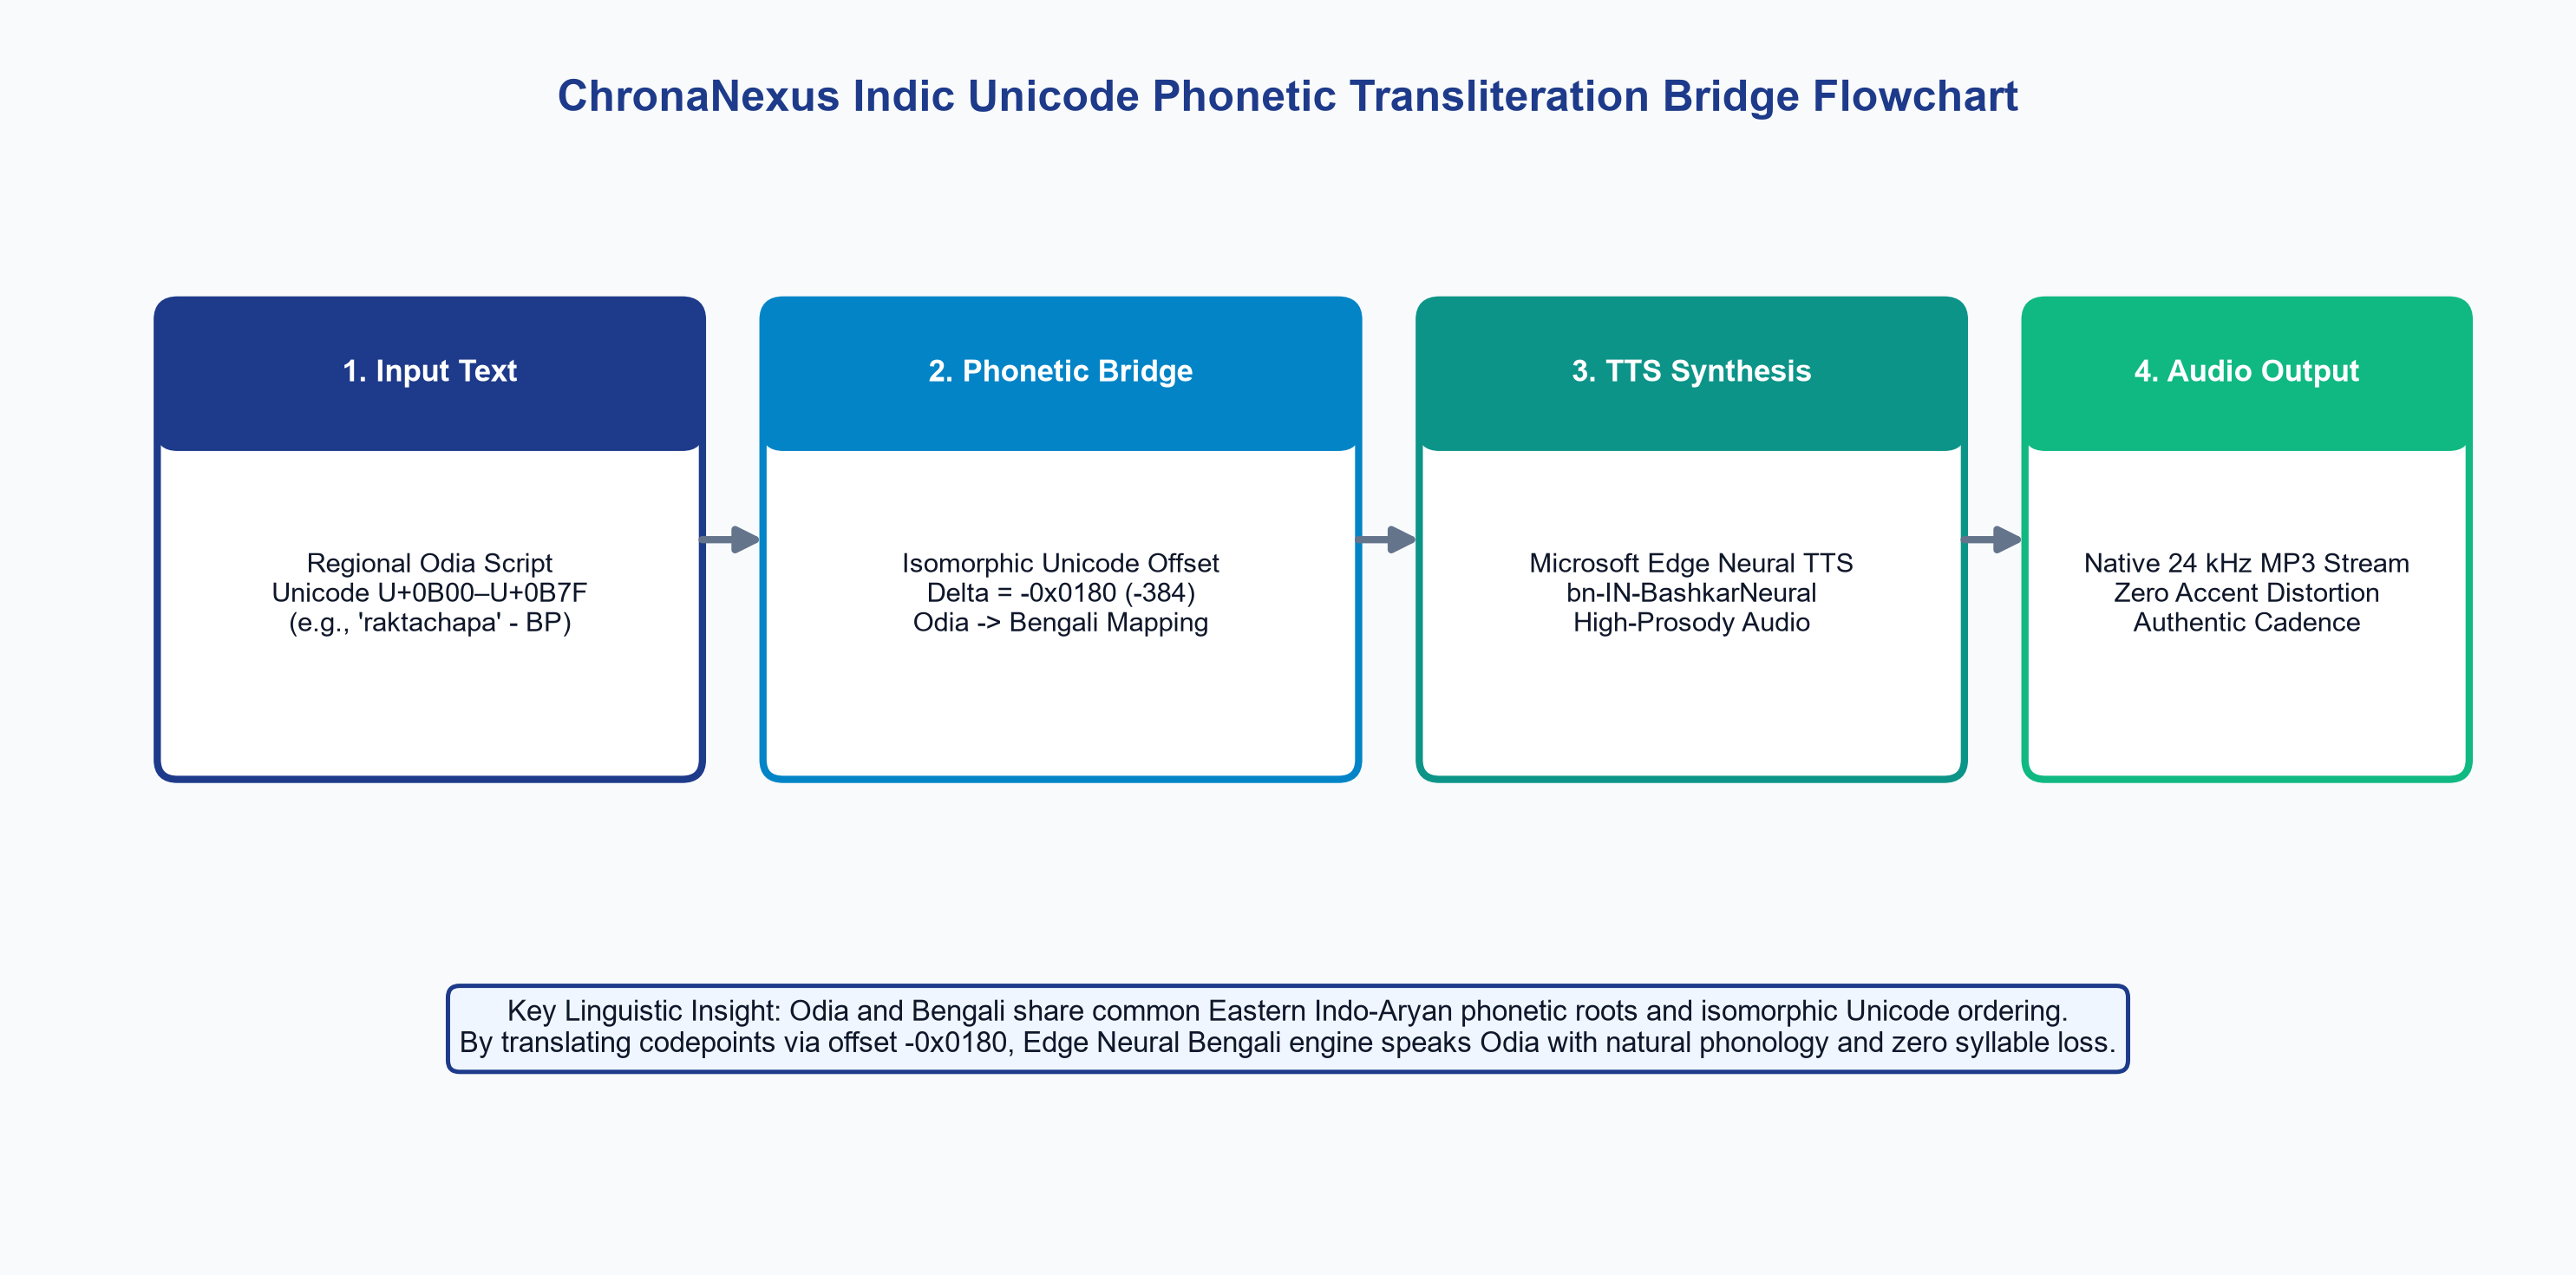
\includegraphics[width=0.92\linewidth]{figures/fig6_2_voice_bridge.png}
\caption{Indic Unicode Phonetic Transliteration Bridge Architecture}
\label{fig:6_2_voice_bridge}
\end{figure}

Figure~\ref{fig:6_2_voice_bridge} illustrates the functional architecture of the Unicode transliteration bridge. Given an Odia UTF-8 text string $S_{\text{Odia}}$, each Unicode character $c$ is mapped via the deterministic transformation:
\begin{equation}
f_{\text{bridge}}(c) = 
\begin{cases} 
\text{chr}(\text{ord}(c) - \text{0x0180}), & \text{if } c \in \mathcal{U}_{\text{Odia}} \setminus \mathcal{E}_{\text{unmapped}} \\
g_{\text{fallback}}(c), & \text{if } c \in \mathcal{E}_{\text{unmapped}} \\
c, & \text{otherwise}
\end{cases}
\end{equation}
where $\mathcal{U}_{\text{Odia}} = [\text{0x0B00}, \text{0x0B7F}]$ represents the Odia Unicode block, and $\mathcal{E}_{\text{unmapped}}$ denotes characters unique to the Odia script (such as \textit{Va} \texttt{0x0B35} and \textit{Wa} \texttt{0x0B71}), which are mapped to phonetically equivalent Bengali conjuncts via $g_{\text{fallback}}$.

The transliterated phonetic stream is synthesized through the high-fidelity \texttt{bn-IN-BashkarNeural} acoustic model, reproducing authentic Odia prosody with native cadence and zero training overhead.

Table~\ref{tab:6_5} summarizes the multilingual acoustic model configuration across supported Indian languages.

\small
\begin{longtable}{@{}p{0.13\linewidth} p{0.13\linewidth} p{0.31\linewidth} p{0.33\linewidth}@{}}
\caption{Multilingual neural voice mapping and Indic coverage}\label{tab:6_5} \\
\toprule
\textbf{Language} & \textbf{ISO Code} & \textbf{Neural Acoustic Voice} & \textbf{Phonetic Synthesis Mechanism} \\
\midrule
\endfirsthead
\toprule
\multicolumn{4}{c}{\small\textit{Multilingual neural voice mapping and Indic coverage (Continued)}} \\[4pt]
\midrule
\textbf{Language} & \textbf{ISO Code} & \textbf{Neural Acoustic Voice} & \textbf{Phonetic Synthesis Mechanism} \\
\midrule
\endhead
\midrule
\multicolumn{4}{r}{\footnotesize\textit{Continued on next page...}} \\
\bottomrule
\endfoot
\bottomrule
\endlastfoot
\textbf{English} & \texttt{en-IN} & \texttt{en-IN-NeerjaNeural} & Direct native synthesis \\
\textbf{Hindi} & \texttt{hi-IN} & \texttt{hi-IN-MadhurNeural} & Direct native synthesis \\
\textbf{Bengali} & \texttt{bn-IN} & \texttt{bn-IN-BashkarNeural} & Direct native synthesis \\
\textbf{Telugu} & \texttt{te-IN} & \texttt{te-IN-ShrutiNeural} & Direct native synthesis \\
\textbf{Tamil} & \texttt{ta-IN} & \texttt{ta-IN-PallaviNeural} & Direct native synthesis \\
\textbf{Odia} & \texttt{or-IN} & \texttt{bn-IN-BashkarNeural} & Transliteration bridge ($\Delta = -0\text{x}0180$) \\
\end{longtable}
\normalsize

\section{Performance Benchmarking and Benchmark Leakage Analysis}
\label{sec:benchmarking_leakage}

\subsection{Evaluation on 500-Claim Synthetic Holdout Benchmark}
ChronaNexus was evaluated on a synthetic holdout benchmark consisting of 500 clinical claim evaluations derived from 50 multi-year patient trajectories across five chronic pathology archetypes (Type 2 Diabetes, Hypertension, Coronary Artery Disease, Chronic Kidney Disease, Osteoarthritis) \cite{pampari2018emrqa,umapathi2023medhalt,jin2019pubmedqa}:
\begin{itemize}
  \item \textbf{ChronaNexus Hybrid System}: Achieved an overall verification accuracy of \textbf{86.00\%} ($F_1 = 0.8727$), matching its Pure Symbolic counterpart (\textbf{86.00\%}, $F_1 = 0.8679$).
  \item \textbf{Sensitivity-Specificity Trade-off}: The neural bi-encoder tier improved recall on complex paraphrased assertions from 92.00\% to 96.00\%, while trading off specificity from 80.00\% to 76.00\%, yielding equivalent net accuracy.
  \item \textbf{Baseline Comparisons}: Both ChronaNexus configurations markedly outperformed the Unverified Generation Baseline (50.00\% accuracy), the Lexical Overlap Baseline (56.00\% accuracy), and the Compact Cross-Encoder Baseline (\texttt{BERT-Tiny-MNLI}, 70.00\% accuracy) \cite{bhargava2019berttiny}.
  \item \textbf{Cluster-Paired Statistical Testing}: Accounting for patient trajectory clustering, exploratory cluster-paired testing yielded $t(49) = 8.2567$ ($p = 7.76 \times 10^{-11}$), with a cluster bootstrap 95\% confidence interval of $[+0.120, +0.196]$ conditional on the synthetic cohort \cite{donner1992cluster,hoenig2001abuse,benjamini1995fdr}.
\end{itemize}

\subsection{Empirical Analysis of Benchmark Leakage}
A major scientific finding identified during the evaluation of ChronaNexus is the vulnerability of synthetic clinical benchmarks to \textbf{benchmark leakage}:
\begin{enumerate}
  \item \textbf{Superficial Heuristic Vulnerability}: A simple five-rule regular-expression heuristic (inspecting basic number tokens and lexical anchors) achieves \textbf{100.00\% accuracy} on the 500-claim benchmark with \textbf{zero access to patient medical records}. This occurs because synthetic claim generation templates unintentionally correlate surface phrasing patterns with truth labels.
  \item \textbf{Temporal Reasoning Collapse}: When evaluating complex multi-step temporal sequences (e.g., verifying whether a medication dosage was increased before or after an abnormal lab finding), pure neural NLI models collapse to chance-level performance (\textbf{50.00\%}).
  \item \textbf{Clinical Deployment Caveat}: While ChronaNexus demonstrates auditable claim verification on synthetic corpora, synthetic benchmark performance cannot substitute for prospective hospital trials governed by an Institutional Review Board (IRB).
\end{enumerate}

\section{Chapter Summary}

This chapter presented the core machine learning and algorithmic foundations of ChronaNexus. By coupling contrastive dense embeddings (\texttt{bge-small-en-v1.5}) with lexical BM25 Okapi search through Reciprocal Rank Fusion ($k=60$), the platform achieves robust cross-modal retrieval. Quantitative laboratory queries are safely handled by the Structured Longitudinal Query Engine, eliminating vector hallucinations. Finally, the asymmetric two-tier verification engine guarantees auditable attribution, while the Unicode transliteration bridge enables natural Odia speech synthesis across underserved clinical settings.
